\documentclass[]{article}
\usepackage[UTF8]{ctex}
\usepackage[a4paper,left=10mm,right=10mm,bottom=10mm,top=10mm]{geometry}
\usepackage{graphicx}
\usepackage{float}
\usepackage{amsmath,amsfonts,amssymb,amsthm}
\usepackage{array,color}
%opening
\title{计算机科学中的数学基础Exercise7}
\author{陈昱衡 521021910939}
\date{\today}

\begin{document}

\maketitle

\section*{Warmup1}
\begin{figure}[H]
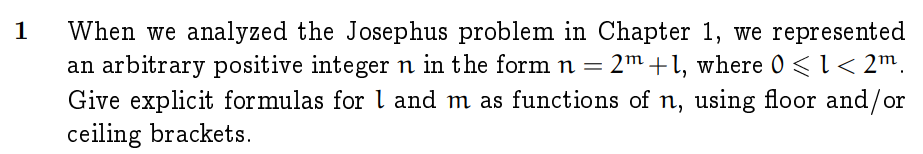
\includegraphics[scale = 1]{Q1.png}
\end{figure}
由$2^m \le n \le 2^m + l$,$0 \le l < 2^m$知,
\begin{equation}
    2^m \le n < 2^{m+1}
\end{equation}
对上式取对数,有:
\begin{align}
    &m \le logn < m+1\\
    &m = \lfloor logn \rfloor \\
    &m + 1 =\lceil logn \rceil 
\end{align}
故,答案为:
\begin{align}
    m &= \lfloor logn \rfloor \\
        &= \lfloor logn \rfloor - 1\\
    l &= n - 2^m\\
        &= n - 2^{\lfloor logn \rfloor}\\
        &= n - 2^{\lceil logn \rceil - 1}
\end{align}



\section*{Warmup2}
\begin{figure}[H]
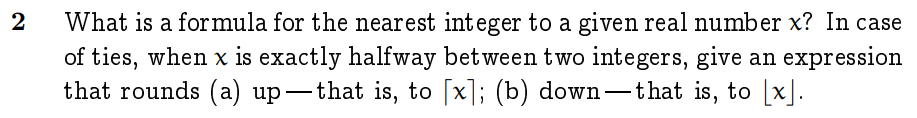
\includegraphics[scale = 1]{Q2.png}
\end{figure}
首先,很容易发现离x最近的整数相当于对x进行四舍五入,当然,*.5的情况有稍微差异。
不妨设离x最近的整数为y,所以很容易写出:
\begin{align}
    (a) \quad y &= \lfloor x+0.5 \rfloor\\
    (b) \quad y &= \lceil x-0.5 \rceil
\end{align}


\section*{Warmup3}
\begin{figure}[H]
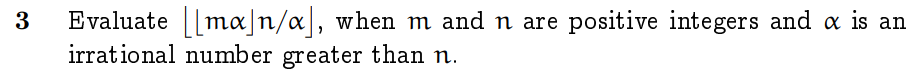
\includegraphics[scale = 1]{Q3.png}
\end{figure}
不妨令:
\begin{align}
    \alpha &= k + {\alpha} \\
    k &= \lfloor k \rfloor
\end{align}
有,
\begin{align}
    \lfloor \frac{\lfloor m\alpha \rfloor n}{n} \rfloor&=\lfloor \frac{(m\alpha - m{\alpha})n}{\alpha} \rfloor \\
    &=mn - \lfloor \frac{mn{\alpha}}{\alpha} \rfloor \\
    &= mn - 1
\end{align}

\section*{Warmup4}
\begin{figure}[H]
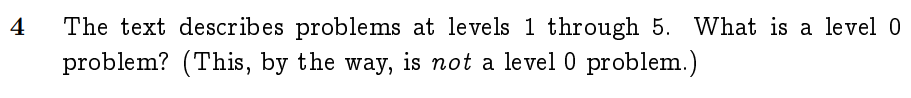
\includegraphics[scale = 1]{Q4.png}
\end{figure}
指不需要给出严谨的证明,可以根据经验、意识、感觉猜测出来的问题。\par 

\section*{Warmup5}
\begin{figure}[H]
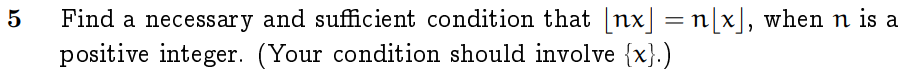
\includegraphics[scale = 1]{Q5.png}
\end{figure}
由定义,有:
\begin{align}
    \lfloor nx \rfloor &= \lfloor n\lfloor x\rfloor + n{x} \rfloor \\
                        &= n\lfloor x \rfloor + \lfloor n{x}\rfloor
\end{align}
根据题意,有:
\begin{align}
    \lfloor nx \rfloor = n\lfloor x \rfloor
\end{align}
故有:
\begin{align}
    \lfloor n\lfloor x\rfloor \rfloor = 0    
\end{align}

因为n为正整数,所以有:
\begin{align}
    &0 \le n{x} < 1\\
    &0 \le {x} < \frac{1}{n}\\
    & {x} < \frac{1}{x}
\end{align}

\section*{Warmup6}
\begin{figure}[H]
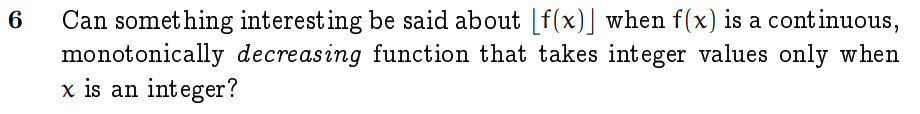
\includegraphics[scale = 1]{Q6.png}
\end{figure}
结论:
\begin{equation}
    \lfloor f(x) \rfloor = \lfloor f(\lceil x \rceil) \rfloor
\end{equation}

由题意,f(x)只在整数处取整数值。因此,不妨令 $\lfloor f(x) \rfloor$ = k,
即,$k \le f(x) < k+1 $,再令 $f(x_{0}) = k$,故由f(x)单调递减,对前述x,有 $\lceil x \rceil = x_{0}$,
有,
\begin{equation}
    \lfloor f(x) \rfloor = \lfloor f(\lceil x \rceil) \rfloor
\end{equation}

\end{document}